\documentclass[11pt,aspectratio=169]{beamer}
 
\usetheme[sectionpage=none, subsectionpage=none, progressbar=none]{metropolis}           % Use metropolis theme
 
  \usepackage{outlines}
  \usepackage{caption}
  \usepackage{appendixnumberbeamer}
  \usepackage{booktabs}
  \usepackage{tcolorbox}
  \usepackage{tabularx}
  \usepackage[export]{adjustbox}[2011/08/13]
  \usepackage{bm}
  
  \def\shrug{\texttt{\raisebox{0.75em}{\char`\_}\char`\\\char`\_\kern-0.5ex(\kern-0.25ex\raisebox{0.25ex}{\rotatebox{45}{\raisebox{-.75ex}"\kern-1.5ex\rotatebox{-90})}}\kern-0.5ex)\kern-0.5ex\char`\_/\raisebox{0.75em}{\char`\_}}}

\usepackage{lmodern}% http://ctan.org/pkg/lm

\newcolumntype{R}{>{\raggedleft\arraybackslash}X} 

\newtheorem*{defn}{Def'n}

  
 \setbeamertemplate{footline}[frame number]{}

\setbeamertemplate{footline}{% 
  \hfill% 
  \usebeamercolor[fg]{page number in head/foot}% 
  \usebeamerfont{page number in head/foot}% 
  \insertframenumber%
  %\,/\,\inserttotalframenumber
  \kern1em\vskip2pt% 
}

\makeatletter
\setbeamertemplate{headline}{%
  \begin{beamercolorbox}[colsep=1.5pt]{upper separation line head}
  \end{beamercolorbox}
  \begin{beamercolorbox}{section in head/foot}
    \vskip2pt\insertnavigation{\paperwidth}\vskip2pt
  \end{beamercolorbox}%
  \begin{beamercolorbox}[colsep=1.5pt]{lower separation line head}
  \end{beamercolorbox}
}
\let\@@magyar@captionfix\relax % IMPORTANT: This is a workaround to fix a random eror with the 2018 installation
\makeatother

\usepackage{xcolor} 
\listfiles

\setbeamercolor{section in head/foot}{fg=normal text.bg, bg=structure.fg}

    \usepackage{smartdiagram}
    \usepackage{tikz}
\usetikzlibrary{shapes.geometric, arrows}
\tikzstyle{startstop} = [rectangle, rounded corners, minimum width=3cm, minimum height=1cm,text centered, draw=black, fill=red!30]
\tikzstyle{io} = [trapezium, trapezium left angle=70, trapezium right angle=110, minimum width=3cm, minimum height=1cm, text centered, draw=black, fill=blue!30]
\tikzstyle{process} = [rectangle, minimum width=3cm, minimum height=1cm, text centered, draw=black, fill=orange!30]
\tikzstyle{decision} = [diamond, minimum width=3cm, minimum height=1cm, text centered, draw=black, fill=green!30]

\title{Gov 2006: Formal Political Theory II \\
Section 7}
\date{\today}
\author{ \textbf{Sophie Hill}}


\begin{document}
  \maketitle
  
 %%%%%%%%%%%%%%%%%%%%%%%%%%%%%%%%%%%%%%%%%%
\begin{frame}{Today}

\Large 

 Citizen candidate model

\begin{itemize}
\item Review the model 
\item Empirical application 1: Chattopadhyay \& Duflo (2004)
\item Empirical application 2: Gro{\ss}er \& Palfrey (2019)
\end{itemize}

\end{frame}

\begin{frame}{Citizen-candidate model}

\begin{itemize}
\item Very influential set of models: ``a conceptualization of a pure form of representative democracy in which government is \textit{by}, as well as \textit{of}, the people."
\pause 
\item Good stuff:
\begin{itemize}
\item Relaxes assumption of commitment and fixed parties
\item Generates policy divergence, 3+ candidate equilibria possible
\end{itemize}
\pause 
\item However, only one election. 
\pause 
\item Osborne \& Slivinski (1996) came first with a simpler model (unidimensional, sincere voting) but Besley \& Coate (1997) is more widely-cited.  \small\shrug


\end{itemize}
\end{frame}

\begin{frame}
\frametitle{Setup: citizens}

\begin{itemize}
\item $N$ citizens denoted $i\in \mathcal{N} = \{1,...,N\}$.
\item Citizen $i$, if elected, implements a policy vector $x\in \mathcal{A}^i$, where $\mathcal{A}=\cup^N_{i=1} \mathcal{A}^i$.
\item $i$ receives utility $V^i(x,j)$ from candidate $j \in \mathcal{N} \cup \{0\}$ implementing $x\in \mathcal{A}$.
\item Anyone can choose to run for office, at cost $\delta > 0$
\item Only citizens who choose to run for office can be elected
\end{itemize}

\end{frame}

\begin{frame}
\frametitle{Setup: institutions}

\begin{itemize}
\item Election decided by plurality vote, with equal probability of each candidate winning where the election is tied: {\it i.e.} only one candidate elected.
\item Voting is costless. 
\item If no candidate stands, default option $x_0 \in \cap_i \mathcal{A}^i$ is implemented.
\end{itemize}

\pause
\begin{tcolorbox}
What does the model assume about commitment?
\end{tcolorbox}

\pause 

\begin{itemize}
\item One-shot election game with full information = no candidate can credibly commit to a policy other than her ideal point in $\mathcal{A}^i$. %(Simple backward induction logic.)
\end{itemize}

\end{frame}



\begin{frame}
\frametitle{Game structure}

Timing: \begin{enumerate}
\item All citizens decide whether to stand for office, $s^i\in\{0,1\}$.
\item All citizens $j$ vote simultaneously by choosing one candidate $i$ from the set of available candidates $\mathcal{C}$, or abstaining: $\alpha_j = i$ or $\alpha_j=0$. 
\item The winning candidate $i$ implements her preferred policy $x^*_i \in  \mathcal{A}^i$.
\end{enumerate}

...so a pure strategy for each $i$ is: $$y^i \equiv (s^i,\alpha^i,x^i) \in \{0,1\} \times \mathcal{C} \cup \{0\} \times \mathcal{A}^i.$$

\end{frame}

\begin{frame}{Solving backward}
Dynamic game of complete information: we look for an SPE by backward induction.

\begin{enumerate}
\item Once a citizen is elected, find the \textbf{policy implemented}.
\item Given a set of candidates (and knowing their bliss points), find the best \textbf{voting choice} for each citizen.
\item Foreseeing what will happen next, citizens decide \textbf{whether to run} or not.
\end{enumerate}

Equilibrium: \textit{set of entry decisions} such that each citizen's decision is optimal given decisions of others and expected voting.

\end{frame}


\begin{frame}
\frametitle{Working backwards: (1) Policy implementation}

After being elected, $i$ maximizes her own utility by choosing her preferred available policy: $$x^*_i = \arg \max_x \{ V^i(x,i)|x\in \mathcal{A}^i \}.$$ Assume $x^*_i$ is unique. % (what assumptions would we need?).

\bigskip

Every citizen $j$ receives utility $V^j(x^*_i,i)\equiv V_{ji}$ from $i$'s policy choice (or $V^j(x_0,0)\equiv V_{j0}$ if no candidate was elected). 

\end{frame}



\begin{frame}
\frametitle{Working backwards: (2) Voting}

Denote the combined vector of votes as $\alpha = (\alpha_1,...,\alpha_N)$. Candidate $i$ receives $\#\mathcal{N}_i$ votes. 

\bigskip

The set of ``winning'' candidates following $\alpha$ is $W(\mathcal{C},\alpha)$. 

\bigskip

The probability of a winning candidate $i\in W(\mathcal{C},\alpha)$ winning the election is therefore: $$P^i(\mathcal{C},\alpha) = \frac{1}{\#W(\mathcal{C},\alpha)}.$$ 

\bigskip

This probability is zero for everyone else. 

\end{frame}



\begin{frame}
\frametitle{Working backwards: (1) Decision to stand}

Vector of decisions to stand $s=(s^1,...,s^N)$. This defines the candidate set $\mathcal{C}(s) = \{i|s^i=1\}$; and thus $\alpha(\mathcal{C}(s))$. 

\bigskip

\pause 
\begin{tcolorbox}
In this model, would a citizen ever run for office if they have no chance of winning?
\end{tcolorbox}

\pause

Yes! Citizens may run in order to win office, but also to prevent someone else from winning to obtain a better outcome (i.e., run as a spoiler).


\end{frame}

\begin{frame}{Working backwards: (1) Decision to stand}

Citizen $j$ thus receives expected utility of $$U^j\bigg(s; \alpha(\mathcal{C})\bigg) = \sum_{i\in\mathcal{C}(s)} P^i\bigg(\mathcal{C}(s), \alpha(\mathcal{C}(s))\bigg)V_{ji} + P^0\bigg(\mathcal{C}(s)\bigg)V_{j0} - \delta s^j,$$

\bigskip

where the terms represent

\begin{enumerate}
\item the weighted policy outcome payoff \\
\item default payoff (if no candidate stands) \\
\item the cost of running
\end{enumerate}



\end{frame}



\begin{frame}
\frametitle{Voting equilibria}

We focus on pure strategy SPNEs. These are defined by: \begin{enumerate}
\item Optimal (strategic) voting $\alpha^*$ such that $\alpha_j^*$ is a best response to $\alpha_{-j}^*$ for all $j$: $$\alpha_j^* \in \arg \max_{\alpha_j} \bigg\{ \sum_{i\in \mathcal{C}(s)} P^i\bigg(\mathcal{C}(s), \alpha_j, \alpha_{-j}^*\bigg)V_{ji} \bigg| \alpha_j \in \mathcal{C}(s) \cup \{0\} \bigg\}$$ and $\alpha_j^*$ is not weakly dominated.%\footnote{Ruling out weakly dominated strategies allows us to get sincere voting in two-candidate elections.} 
\item Each citizen $i$ chooses $s_i^*$ anticipating $\alpha^*(\mathcal{C}(s_i,s^*_{-i}))$. 
\end{enumerate}

\end{frame}



\begin{frame}
\frametitle{Conditions for equilibria}

%\begin{footnotesize}
%Voting is not mechanistic given $\mathcal{C}$---many possible voting equilibria that can arise for any given $s^*$ (esp. with $\#\mathcal{C}>2$). 

%Approach: we focus on $s^*$ and choose $\alpha^*$ to support SPNEs. 



Two central incentives/conditions for standing:

\pause 


\begin{enumerate}
\item \textbf{Participation}: $i \in \mathcal{C}(s)$ must \textbf{want} to stand: \begin{footnotesize}\begin{eqnarray*}
&& \sum_{j \in \mathcal{C}(s)} P^j\bigg(\mathcal{C}(s), \alpha(\mathcal{C}(s))\bigg)V_{ij} -\delta \geq \\ 
&& \sum_{j \in \mathcal{C}(s)/\{i\}} P^j\bigg(\mathcal{C}(s)/\{i\}, \alpha(\mathcal{C}(s)/\{i\})\bigg)V_{ij} + P^0\bigg(\mathcal{C}(s)/\{i\}\bigg)V_{i0}.
\end{eqnarray*} \end{footnotesize}

\pause 
\item \textbf{Entry proofness}: \textbf{no other citizen} $i\not\in\mathcal{C}(s)$ wants to become a candidate (to either win or spoil): \begin{footnotesize}\begin{eqnarray*}
&& \sum_{j \in \mathcal{C}(s)} P^j\bigg(\mathcal{C}(s), \alpha(\mathcal{C}(s))\bigg)V_{ij} + P^0\bigg(\mathcal{C}(s)\bigg)V_{i0} \geq \\
&& \sum_{j \in \mathcal{C}(s)\cup\{i\}} P^j\bigg(\mathcal{C}(s)\cup\{i\}, \alpha(\mathcal{C}(s)\cup\{i\})\bigg)V_{ij} - \delta.
\end{eqnarray*} \end{footnotesize}
\end{enumerate}

\end{frame}



\begin{frame}
\frametitle{Sincere partitions}

Before (finally) characterizing equilibria, let's define a \textbf{sincere partition}. A given partition $\{ \mathcal{N}_i \}_{i\in \mathcal{C}\cup \{0\}}$ is sincere iff: 
\begin{enumerate}
\item $k\in \mathcal{N}_i$ implies $V_{ki}\geq V_{kj}, \forall j\in\mathcal{C}$. 
\item $k\in \mathcal{N}_0$ implies $V_{ki} = V_{kj}, \forall i,j\in\mathcal{C}$. 
\end{enumerate}

\bigskip

In human words: this divides the electorate among the candidates, so that each $k$ is associated with her preferred candidate $j$, or the status quo if indifferent between all candidates.

\bigskip

\pause

\begin{tcolorbox}
Is a sincere partition unique for a given set of voters \& candidates?
\end{tcolorbox}

\pause 

No! Since voters may be indifferent, they can be many possible sincere partitions.

%Given voters may be indifferent, there may be many possible sincere partitions.

%\bigskip 

% Sincere partitions tell us who will win -- i.e. defines $W(\mathcal{C},\alpha)$.

\end{frame}



\begin{frame}
\frametitle{One candidate equilibrium}

$i$ runs unopposed iff: \begin{enumerate}
\item \textbf{Participation}: $V_{ii}-V_{i0} \geq \delta$.
\item \textbf{Entry proofness}: for all $k \in \mathcal{N}/\{i\}$ such that $\#\mathcal{N}_k \geq \#\mathcal{N}_i$ for all sincere partitions $(\mathcal{N}_i,\mathcal{N}_k,\mathcal{N}_0)$, we have \vspace{-8pt}$$\frac{1}{2}(V_{kk}-V_{ki}) \leq \delta$$ if there exists a sincere partition such that $\#\mathcal{N}_k = \#\mathcal{N}_i$, and $$V_{kk}-V_{ki}\leq \delta$$ if $\#\mathcal{N}_k > \#\mathcal{N}_i$.
\end{enumerate}

\bigskip

So, $i$ must want to stand unopposed, and any $k$ who could at least tie finds it too costly.

\end{frame}


\begin{frame}
\frametitle{What does this mean?}

$\delta$ high: entry proofness easy to satisfy, but participation constraint means that the candidate running is an extremist (relative to the status quo). 

\bigskip
\pause 

$\delta$ low: participation condition easy to satisfy, and entry proofness guaranteed by a centrist candidate attracting a lot of support. As $\delta\rightarrow 0$, for $i$ to run unopposed she must be a Condorcet winner. 

\end{frame}



\begin{frame}
\frametitle{Two candidate equilibrium}

Only candidates $i$ and $j$ compete iff: \begin{enumerate}
\item Both can win (so are tied): there exists a sincere partition $(\mathcal{N}_i,\mathcal{N}_j,\mathcal{N}_0)$ such that $\#\mathcal{N}_i = \#\mathcal{N}_j$.
\item \textbf{Participation}: $\frac{1}{2}(V_{ii}-V_{ij}) \geq \delta$ and $\frac{1}{2} (V_{jj}-V_{ji}) \geq \delta$.
\item \textbf{Entry proofness}: $\#\mathcal{N}_0 +1 < \#\mathcal{N}_i=\#\mathcal{N}_j$.
\end{enumerate}

\bigskip

\begin{itemize}
\item In the two candidate equilibrium, both candidates must have a chance of winning. \alert{Why?} \pause Citizens always vote sincerely in a 2-candidate race, so no point in running as a spoiler. \pause 
\item When is \alert{(2)} satisfied? \pause Distinct candidates or high office rents. \pause
\item What if a \alert{third candidate} enters? \pause $i$'s voters would not defect to a third candidate $k$ even if they preferred her, for fear of allowing $j$ to win (and vice versa).

\end{itemize}

In words: candidates must have some chance of winning. We either have high office rents and centrist candidates, or two different types of candidate. And we need that $i$'s supporters would not switch to $k$ if they entered, since this would make $j$ win.

\end{frame}


\begin{frame}
\frametitle{Three or more candidate equilibrium}

\begin{footnotesize}

Take a SPNE $(s^*, \alpha^*(\mathcal{C}(s^*)))$ where $\#\mathcal{C}(s^*)\geq 3$, with associated winning set $\hat{W}(s^*)\geq 2$. Given a sincere voting partition over $\hat{W}(s^*)$, for any winning candidate $i,j\in \hat{W}(s^*)$:  \begin{enumerate}
\item All winning candidates tie: $\#\mathcal{N}_i = \#\mathcal{N}_j, \forall i, j \in \hat{W}(s^*)$.
\item Voters (including candidates) prefer the lottery over winners to their next most preferred candidate: for all $i \in \hat{W}(s^*)$,\vspace{-8pt} $$\sum_{j\in \hat{W}(s^*)} \left( \frac{1}{\#\hat{W}(s^*)}\right) V_{\ell j} \geq \max \bigg\{ V_{\ell j} \bigg| j \in \hat{W}(s^*)/\{i\} \bigg\}, \forall \ell \in \mathcal{N}_i.$$ 
\end{enumerate} For every losing candidate $k\in \mathcal{C}(s^*)/\hat{W}(s^*)$: \begin{enumerate}
\item $k$'s candidacy affects outcome: $\hat{W}(\mathcal{C}(s^*)/\{k\}, \alpha(\mathcal{C}(s^*)/\{k\})) \neq \hat{W}(s^*)$. 
\item Participation (of $k$): there exists an $h \in \mathcal{C}(s^*)$ such that: $$\sum_{i\in \hat{W}(s^*)} \left( \frac{1}{\#\hat{W}(s^*)}\right) V_{ki} - \delta > V_{kh}.$$
\end{enumerate}

\end{footnotesize}

%\vspace{-10pt} These are easy to construct by choosing our voting equilibria. 

\end{frame}



\begin{frame}
\frametitle{Costs and benefits of this approach}

Benefits: \begin{enumerate}
\item Realism in terms of entry and commitment.
\item Rationalizes median divergence. 
\item Political equilibria directly derived from the primitives: the set of possible policies that are given by the available policy technology, and citizens' preferences over these policies. 
\end{enumerate}

\bigskip

Costs: \begin{enumerate}
\item Many equilibria, so hard to make predictions about number of candidates and especially policy outcomes. 
\item Some assumptions seem stringent: complete information and a one-shot game.
\end{enumerate}

\end{frame}

\begin{frame}
\frametitle{Chattopadhyay \& Duflo (2004)}

\begin{itemize}
\item Empirical application of the citizen candidate model
\item Village councils in India which have authority over local public goods decisions.
\item Government mandated that one-third of council heads be women, and randomly allocated which ones were women.
\item Key question: how do reservations affect policy equilibria? 
\begin{itemize}
\item MVT: political decisions reflect median voter
\item C-C: identity of candidate matters for outcomes
\end{itemize}
\item Find that reservations substantively affect public goods allocation decisions ``in ways that seem to better reflect women's preferences"
\end{itemize}

\end{frame}

\begin{frame}
\frametitle{Setup}

\begin{itemize}
\item Unidimensional competition: $\mathcal{A}_i=[0,1], \forall i\in\mathcal{N}$. Default $\mu'$.
\item Euclidean preferences, no office motivation: $V^i(x,j) = -|\omega_i - x|$. Denote median by $m$.
\item For women, $\omega_i\in[0,W]$; for men, $\omega_i\in[M,1]$. And $\delta_M<\delta_W$. 
\begin{itemize}
\item Think of this as social costs of candidacy being higher for women.
\end{itemize}
\item Local powers also matter: $x_j = \alpha \omega_j + (1-\alpha) \mu'$.
\begin{itemize}
\item C\&D motivate this as elite capture or lobbying by village assembly.
\item Justifies the assumption that $\mu' > m$.
\end{itemize}
\end{itemize}

\bigskip

\begin{itemize}
\item Parameters may be such that \textit{no equilibrium} exists where a woman is a candidate without reservations $\rightarrow$ outcome will be greater than $M$.
\item Reservations $\rightarrow$ shift policy outcomes to the left -- improves women's utility, often median utility.
\end{itemize}

\end{frame}



\begin{frame}
\frametitle{Equilibrium with no female candidates}

\textbf{Proposition 1.} No women ever runs for office (without a reservation) when: \begin{enumerate}
\item No woman would run unopposed: $\delta_W - \frac{\delta_M}{2} > \mu' - m$.
\item No woman would run against a man: $\delta_W > m - (1-\alpha)\mu'$.
\end{enumerate}

\bigskip

%Intuition for 1: with $\delta_W$ high, only women with extreme preferences will run. With $\delta_M$ low, man enters and wins.

%\medskip

Proof of Condition 1: 
\begin{enumerate}
\item Woman runs if $\mu' - x_j \geq \delta_W$.
\item Woman most likely to defeat man is $x_j^W = \mu'-\delta_W$.
\item A man runs against this woman if $x_j^M \geq \delta_M + x_j^W = \delta_M + \mu' - \delta_W$, and wins if $x_j^M - m < m - x_j^W$.
\item Substituting in for $x_j^M$ and $x_j^W$ yields the condition.
\end{enumerate}

\end{frame}


\begin{frame}\frametitle{Equilibrium with no female candidates}

\textbf{Proposition 1.} No women ever runs for office (without a reservation) when: \begin{enumerate}
\item No woman would run unopposed: $\delta_W - \frac{\delta_M}{2} > \mu' - m$.
\item No woman would run against a man: $\delta_W > m - (1-\alpha)\mu'$.
\end{enumerate}

\bigskip

Proof of Condition 2: 
\begin{enumerate}
\item Need symmetry around median for a tie.
\item Most extreme woman at 0 would implement $x_j^0=(1-\alpha)\mu'$.
\item Therefore largest possible distance is $2(m-x_j^0)$.
\item The most extreme woman would never run if $\frac{1}{2}2(m-x_j^0)>\delta_W$.
\item Substituting in $x_j^0$ yields the result.
\end{enumerate}

\end{frame}


\begin{frame}
\frametitle{Empirical results}

Under these conditions, no woman stands, so policy is male-biased. Reservations help by restricting the set of candidates.

\bigskip

Go on to test whether reservations move policy toward female preferences (defined empirically by types of complaints: women care more about welfare and drinking water, men care more about public works) in West Bengal and Rajasthan. 

\bigskip

Comparing reserved to non-reserved, find number of drinking water facilities increased while road quality increased/declined depending on district. 

\end{frame}

\begin{frame}{Gro{\ss}er \& Palfrey (2019)}

\begin{itemize}
\item Lab experiment to test some of the core predictions of the citizen candidate model
\item Model with \alert{incomplete information}: citizen ideal points are i.i.d. but each citizen only knows their own with certainty
\item In another version, citizens receive ideological ``party cues'' informing them of the general position of the candidates (left vs right) but not their exact ideal points.
\end{itemize}

\end{frame}

\begin{frame}{Gro{\ss}er \& Palfrey (2019)}

Use the model to generate lots of precise testable implications... for example: 

\begin{itemize}
\item More extreme citizens (vs the median) are more likely to run as candidates
\item Entry rates are decreasing in electorate size
\item Entry rates are decreasing in cost of running
\end{itemize}

Lab experiment finds empirical support for all hypotheses! 

\end{frame}

\begin{frame}{Gro{\ss}er \& Palfrey (2019)}

\begin{figure}
\centering
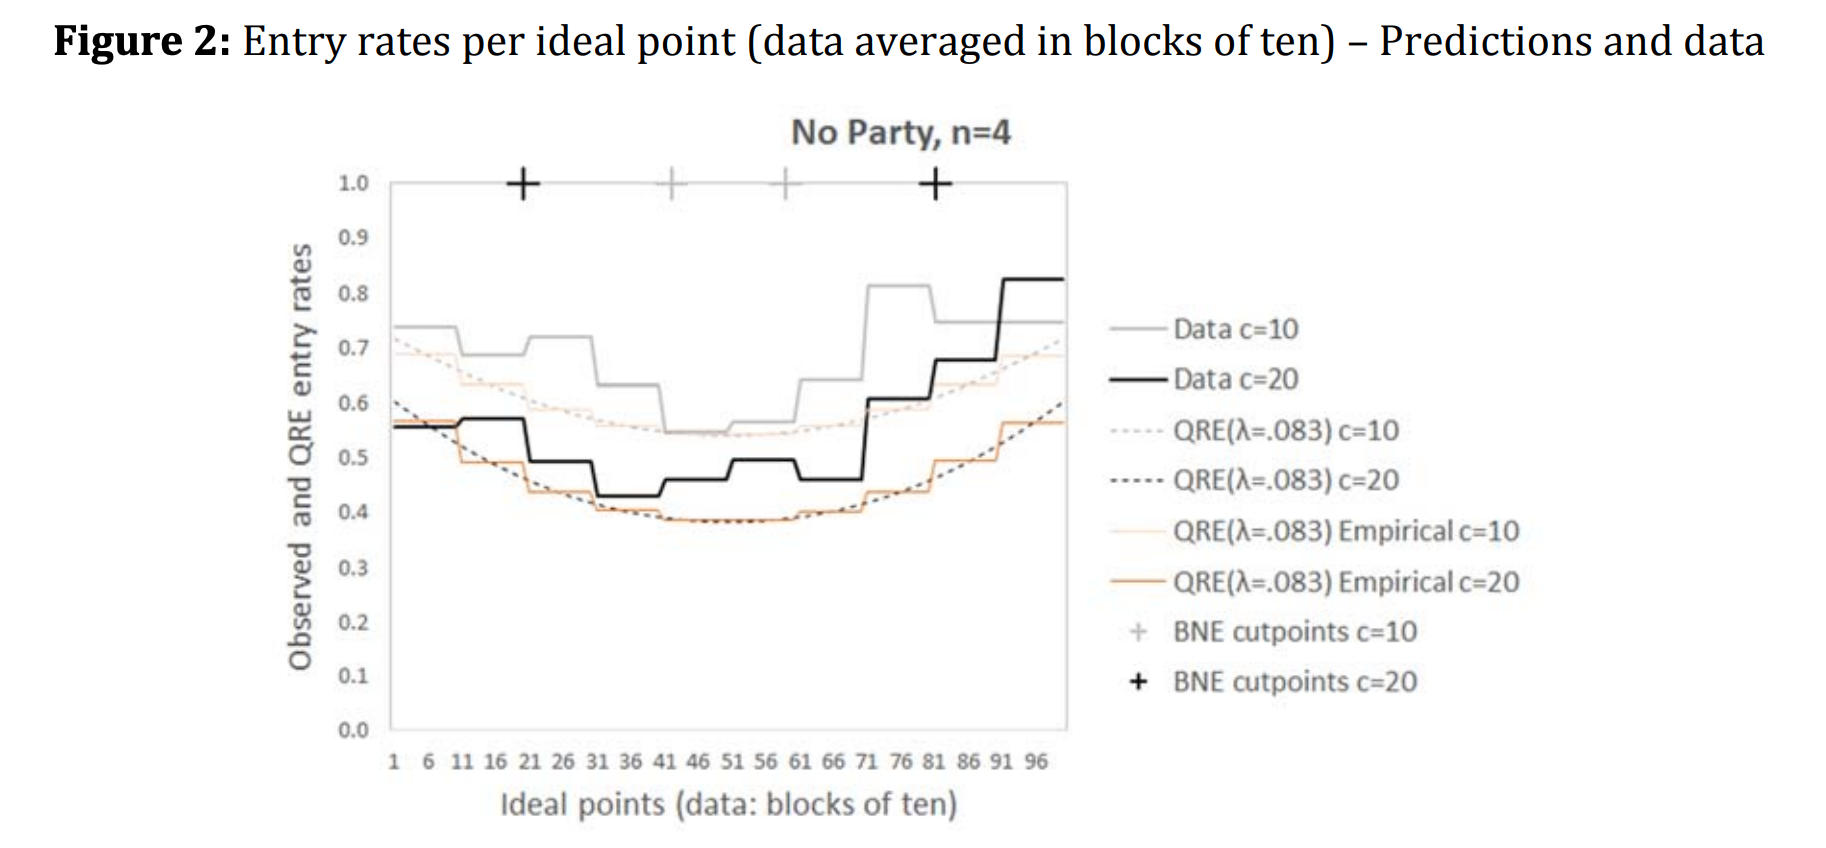
\includegraphics[width=\textwidth]{palfrey.png}
\end{figure}

\end{frame}


\end{document}
